
% This LaTeX was auto-generated from MATLAB code.
% To make changes, update the MATLAB code and republish this document.

\documentclass{article}
\usepackage{graphicx}
\usepackage{color}
\usepackage{amsmath}
\usepackage{amssymb}
\usepackage[a4paper, total={6in,8in}]{geometry}
\usepackage{pdfpages}
\usepackage{multicol}

\sloppy
\definecolor{lightgray}{gray}{0.5}
\setlength{\parindent}{0pt}

\begin{document}

% 
\includepdf{../TitlePage.pdf}

\subsection*{\#2(a)}

\begin{verbatim}
clear;clc;close all
[x, y] = meshgrid(0:0.01:1,0:0.01:1);
len = size(x);
phi_12 = sin(1*pi*x).*sin(2*pi*y);
phi_21 = sin(2*pi*x).*sin(1*pi*y);
phi_13 = sin(1*pi*x).*sin(3*pi*y);
phi_31 = sin(3*pi*x).*sin(1*pi*y);

figure()
surf(x,y,phi_12, 'edgecolor', 'none')
title("$\phi_{12}$ 3D Plot", "fontsize", 14, "interpreter", "latex")
figure()
surf(x,y,phi_21, 'edgecolor', 'none')
title("$\phi_{21}$ 3D Plot", "fontsize", 14, "interpreter", "latex")

figure()
contour(x,y,phi_12,'ShowText','on')
title("$\phi_{12}$ 2D Plot", "fontsize", 14, "interpreter", "latex")
figure()
contour(x,y,phi_21,'ShowText','on')
title("$\phi_{21}$ 2D Plot", "fontsize", 14, "interpreter", "latex")
\end{verbatim}

\begin{figure}[h!]
   \begin{multicols*}{2}
      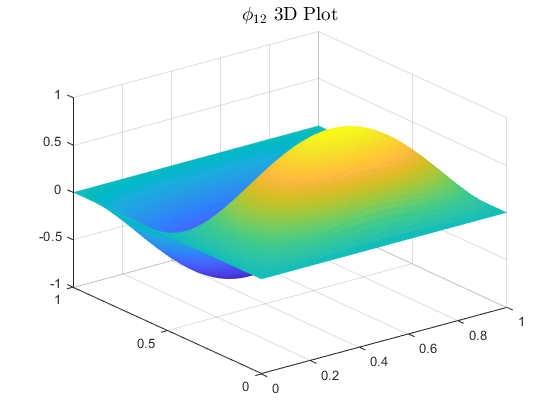
\includegraphics [width=3in]{Untitled4_01.png}

      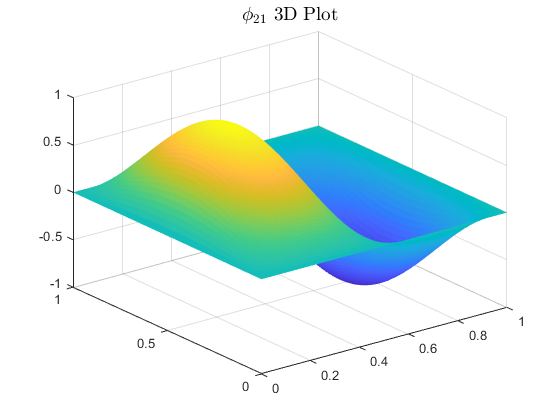
\includegraphics [width=3in]{Untitled4_02.png}

      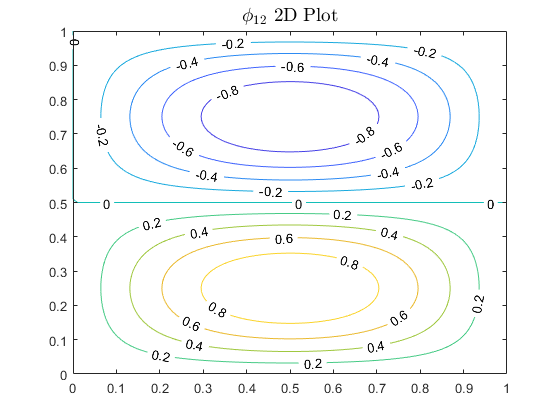
\includegraphics [width=3in]{Untitled4_03.png}

      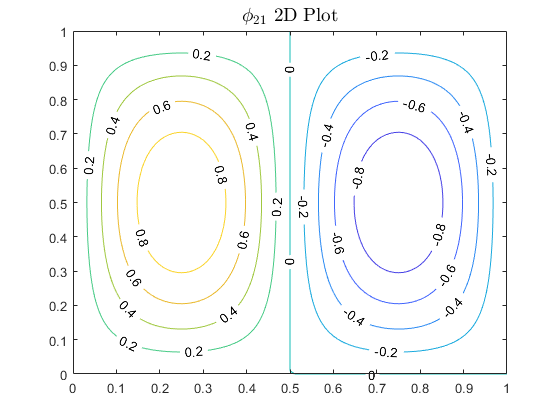
\includegraphics [width=3in]{Untitled4_04.png}
   \end{multicols*}
\end{figure}
\newpage

\subsection*{\#2(b)(c)(d)(e)}

\begin{verbatim}
clear;clc;close all
[x, y] = meshgrid(0:0.01:1,0:0.01:1);
len = size(x);
phi_12 = sin(1*pi*x).*sin(2*pi*y);
phi_21 = sin(2*pi*x).*sin(1*pi*y);
phi_13 = sin(1*pi*x).*sin(3*pi*y);
phi_31 = sin(3*pi*x).*sin(1*pi*y);

figure()
surf(x,y,phi_12+phi_21, 'edgecolor', 'none')
title("$\phi_{12}+\phi_{21}$ 3D Plot", "fontsize", 14, "interpreter", "latex")
figure()
surf(x,y,phi_13+phi_31, 'edgecolor', 'none')
title("$\phi_{13}+\phi_{31}$ 3D Plot", "fontsize", 14, "interpreter", "latex")
figure()
surf(x,y,phi_13-phi_31, 'edgecolor', 'none')
title("$\phi_{13}-\phi_{31}$ 3D Plot", "fontsize", 14, "interpreter", "latex")
figure()
surf(x,y,phi_13+phi_31/3, 'edgecolor', 'none')
title("$\phi_{13}+\frac{1}{3}\phi_{31}$ 3D Plot", "fontsize", 14, "interpreter", "latex")

figure()
contour(x,y,phi_12+phi_21,'ShowText','on')
title("$\phi_{12}+\phi_{21}$ 2D Plot", "fontsize", 14, "interpreter", "latex")
figure()
contour(x,y,phi_13+phi_31,'ShowText','on')
title("$\phi_{13}+\phi_{31}$ 2D Plot", "fontsize", 14, "interpreter", "latex")
figure()
contour(x,y,phi_13-phi_31,'ShowText','on')
title("$\phi_{13}-\phi_{31}$ 2D Plot", "fontsize", 14, "interpreter", "latex")
figure()
contour(x,y,phi_13+phi_31/3,'ShowText','on')
title("$\phi_{13}+\frac{1}{3}\phi_{31}$ 2D Plot", "fontsize", 14, "interpreter", "latex")
\end{verbatim}

\begin{figure}[h!]
   \begin{multicols*}{2}
      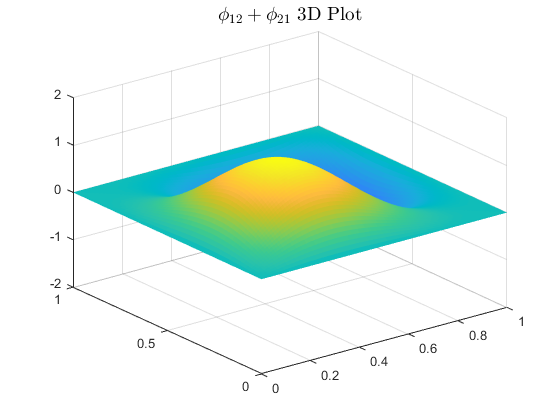
\includegraphics [width=3in]{Untitled4_05.png}

      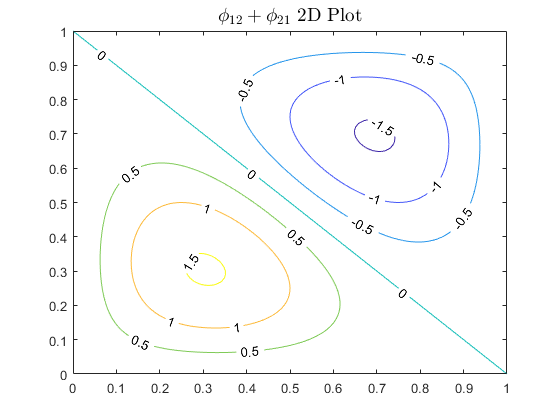
\includegraphics [width=3in]{Untitled4_09.png}
   \end{multicols*}
\end{figure}

\begin{figure}[h!]
   \begin{multicols*}{2}
      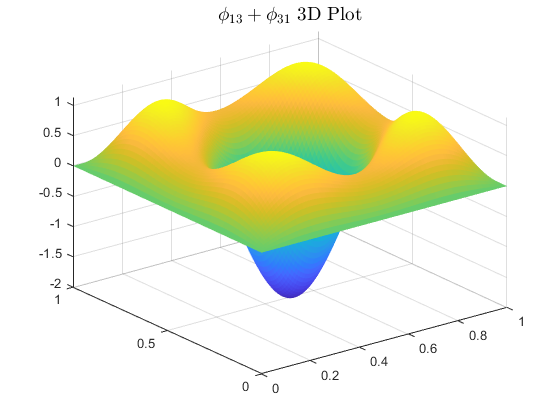
\includegraphics [width=3in]{Untitled4_06.png}

      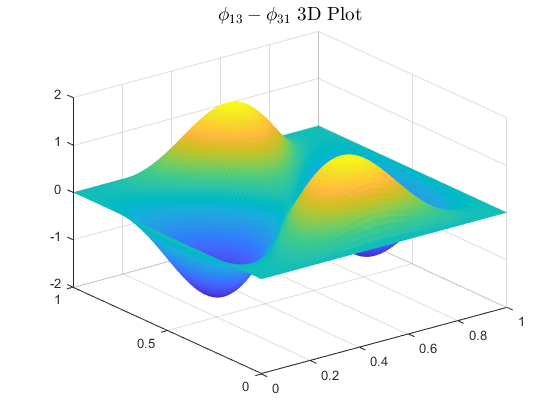
\includegraphics [width=3in]{Untitled4_07.png}

      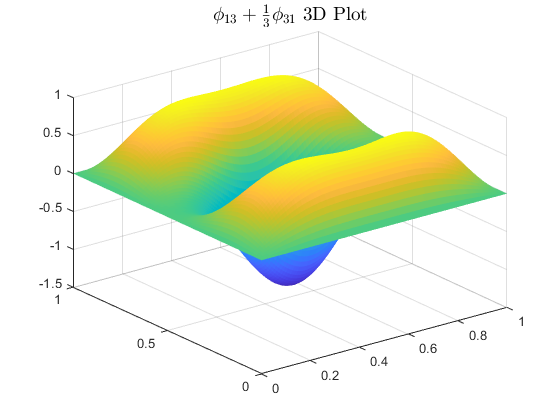
\includegraphics [width=3in]{Untitled4_08.png}

      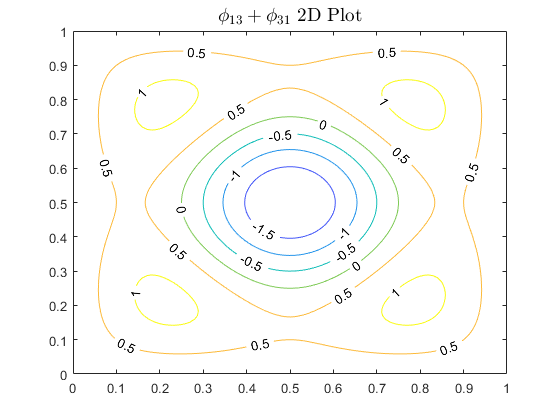
\includegraphics [width=3in]{Untitled4_10.png}

      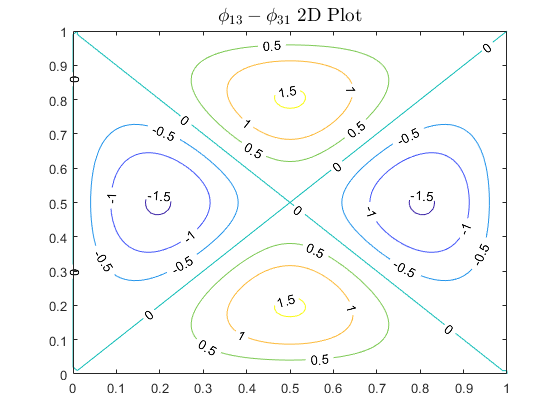
\includegraphics [width=3in]{Untitled4_11.png}

      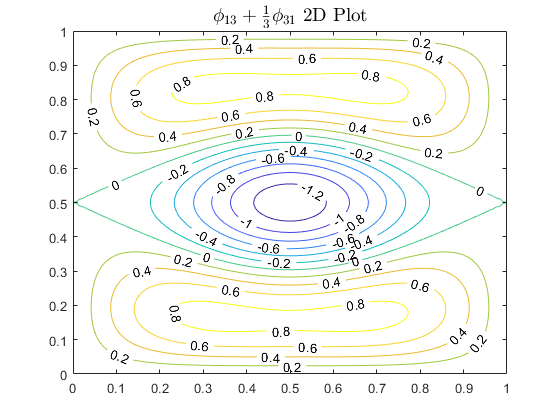
\includegraphics [width=3in]{Untitled4_12.png}
   \end{multicols*}
\end{figure}
\newpage

\hrulefill
   \begin{verbatim}
   clear;clc;close all
   syms x c1 c2
   y = c1*x*(pi/2-x)+c2*x^2*(pi/2-x);
   I = int(2*x*y-y^2+diff(y,x)^2, x, 0, pi/2);

   I_c1 = diff(I,c1);
   I_c2 = diff(I,c2);

   result = vpasolve([I_c1==0; I_c2==0], [c1 c2]);
   c1_ = result.c1
   c2_ = result.c2
   I_min = vpa(subs(I, [c1, c2], [c1_, c2_]))
   \end{verbatim}

           \color{lightgray} \begin{verbatim}
   c1_ =

   -0.38226308020454397830452040163668


   c2_ =

   -0.17706905679930450830512698974608


   I_min =

   -0.27860356386806082489265488067732

   \end{verbatim} \color{black}


\end{document}

